% !TEX root = sn1604_wifes.tex

\begin{figure*}[tb!]
   \centering
   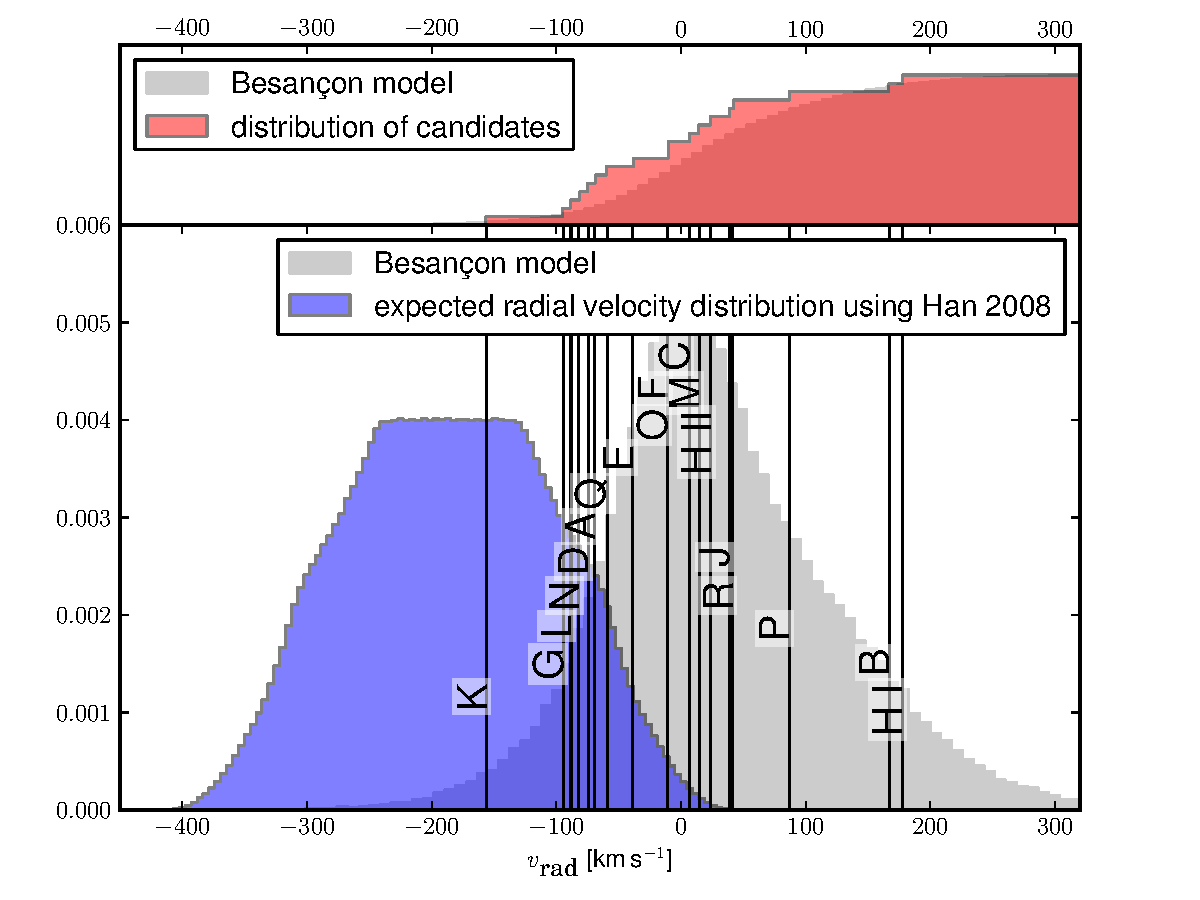
\includegraphics[width=\textwidth]{\plotdir /sn1604_besancon.pdf} 

   \caption{Comparison of \gls{besancon} (1 square degree around Kepler, V cut between 15 and 20) and \citet{2008ApJ...677L.109H} and our measured values. The top panel shows the cumulative distribution for the \gls{besancon} and our measured values. The \citet{2008ApJ...677L.109H} distribution are the result of a Montecarlo simulation including the distribution of random angles and two \citet{2008ApJ...677L.109H} distributions}
   \label{fig:sn1604_besancon}
\end{figure*}


